\documentclass[
%master, % Master version, default: Bachelor   
%cover,  % Custom cover page, must be provided as an coverpage.pdf in A4 size
        % Default: HiØ standard thesis titlepage
%word,   % Word-like paragraph formatting, no indentations, air between paragraphs
        % Default: As all documents are formatted, except those made with default M$ documents
%sans    % Standard HiØ font: Source Sans Pro
        % Default: Computer Modern, designed by Donald Knuth.
]{thesistemplate}

\usepackage[norsk]{babel} % Add this if you use another language
% For available languages and their codes, see https://ctan.org/pkg/babel-contrib

% For those who needs code listings
\usepackage{listings} % DO NOT CHANGE
\renewcommand{\lstlistlistingname}{Kode} % If you are using another language, you need to specify the corresponding "Code List" title

%Metadata, to appear on the half-title page (and the coverpage, if not a custom cover is provided), to be changed by you:

\doctype{Bacheloroppgave} 
\department{Avdeling for Informasjonsteknologi} 
\affiliation{Høgskolen i Østfold} 
\place{Halden} 
\title{The Perfect Thesis} % Main title
\subtitle{Structure, Content and Layout} 
\author{Gunnar Misund}

\RequirePackage{glossaries}
\makeglossaries


\newglossaryentry{latex}
{
    name=latex,
    description={A mark up language specially suited 
    for scientific documents.\LaTeX\ was developed by Leslie Lamport in 1984, and is basically a collection of macros written in \TeX, invented by Donald Knuth, one of the giants of computer science}
}

\newglossaryentry{maths}
{
    name=mathematics,
    description={Mathematics is what mathematicians do}
}




    % OPTIONAL, goes with \printglossaries at the end

%\usepackage{listings}
\begin{document}

\maketitle          % DO NOT CHANGE 
\makehalftitle      % DO NOT CHANGE 
\frontmatter        % All stuff before Introduction: DO NOT CHANGE



\chapter*{About this template}
\label{chap:about}

This document, along with the source code, is meant to be a self-explanatory template for a bachelor's or master's thesis in computer science\footnote{By minor modifications it could be used in any field of research}. It is implemented in \LaTeX, the most popular, advanced, and comprehensive documentation system in mathematics and natural sciences. However, the report as such could be implemented with other tools, as well.

The suggested structure is based on the widely used IMRAD model (Introduction, Methods, Results, And Discussion)\footnote{\url{en.wikipedia.org/wiki/IMRAD}}. The student may of course deviate from the structure and recommended content for each chapter. In particular, the chapters describing the main bulk of work done in the research project (Chapters \ref{chap:design}, \ref{chap:implementation}, and \ref{chap:evaluation}), should be customized to fit the specific topic of your project, both regarding chapter titles and content. You may also, of course, consider merging some of the chapters, and/or add more chapters.

The report is based on the author's personal experiences as a research scientist and lecturer during the last 25 years\footnote{\url{www.ia.hiof.no/~gunnarmi}}, various online resources, 
and the ``The Mayfield Handbook of Technical and Scientific Writing"\cite{perelman97mht}\footnote{\url{www.mhhe.com/mayfieldpub/tsw/home.htm}}.

For technical details, see Chapter \ref{chap:how-to}.

Finally: Comments, bug reports, and suggestions are highly welcome\footnote{\url{gunnar.misund@hiof.no}}!

\vspace{20mm}

Gunnar Misund

Halden, \today





\chapter*{Abstract}
\label{chap:abstract}

An abstract is a brief summarizing statement, not more than one page. It gives the reader a synopsis of the research problem, method, results, and conclusions of your document. The abstract takes the form of a single paragraph and should not contain cross references or citations. Abstracts are sometimes collected into volumes and must be able to stand alone. They may be read by parties trying to decide whether or not to read the main document, or for getting a broad picture before starting on the report. If you describe the content of each main chapter, and bind it nicely together, you’re done. You should not have any information in the abstract that is not found in any of the main chapters. It is common to close the abstract with a few well carefully selected keywords. Obviously, the abstract is the last thing you do in your project. 

Here is an example of a short and concise abstract \cite{winger12e3s}:

\begin{quotation}
\noindent  This thesis presents an evaluation of a set of 3D Scene Graph APIs for Java. The work consists mainly of two parts: Defining a methodology for comparing the APIs, and then applying the proposed methodology to the APIs.
An overview of the available 3D Scene Graph APIs in Java is presented, and a selection of these are chosen for the evaluation. The APIs subjected to the evaluation are Java 3D, Ardor3D and jMonkeyEngine3.
The proposed methodology focuses on the comparison on four different aspects. These are: \textit{Project Management and Technical Infrastructure, System Architecture, System Features and Capabilities, and System Performance}.
The results from applying the evaluation method show that none of the APIs were superior to the others in all respects. The results identify strengths and weaknesses with each API, that indicate which use cases each API might be better suited for.
\newline 
\paragraph{Keywords:} Scene Graph, API, Evaluation, Java, 3D Graphics, OpenGL, Java3D, jMonkeyEngine3, Ardor3D
\end{quotation}




\chapter*{Acknowledgments}
In a thesis, it is common to mention the assistance of
people whose help was crucial but not extensive enough to warrant
their being listed as co-authors. Thesis advisors, technicians, and
colleagues  who gave advice or time are all candidates for the
acknowledgments section. Patient family members are also frequently thanked.


\chapter*{Prerequisites (Optional)}
You may say something about what kind of knowledge and background the reader should have to get the most from reading your thesis.    % OPTIONAL 

\tableofcontents    % DO NOT CHANGE   

\listoffigures      % OPTIONAL 
\listoftables       % OPTIONAL 
\lstlistoflistings  % OPTIONAL 
  
\mainmatter  %Setting the format and layout for all the stuff from Introduction and on: DO NOT CHANGE

% Your chapter files

\chapter{Introduction}
\label{chap:intro}

Chess-playing robots represent a fascinating intersection of robotics, computer spacial recognition, and artificial intelligence. These systems combine mechanical precision with computational intelligence to create machines capable of engaging in one of humanity's oldest strategic games. While chess computers have famously defeated grandmasters since the late 1990s, the physical manipulation of chess pieces by robotic systems presents unique engineering challenges beyond pure computational play.

\section{Background and motivation}
\label{sec:background-motivation}

The development of chess-playing robots has evolved along several technological paths. Previous research has explored various approaches for piece detection and movement systems. For instance, solutions demonstrate a vision-based detection system using overhead cameras to identify piece positions and a robotic arm for movement, while other papers also shed light on systems utilizing magnetic sensors with various movement mechanism for piece manipulation.
Our project aims to combine the strengths of these approaches while introducing novel elements. By implementing hall effect sensors for piece detection and integrating an articulated robotic arm for movement, we create a system that offers reliable position tracking without the lighting dependencies of vision systems, while maintaining the flexibility of a multi-axis robotic manipulator for piece movement.

TODO: Further elaboration needed on the specific advantages of hall effect sensors over camera-based solutions and why this approach is interesting

\subsection{Research question/Problem statement/Objectives}
\label{sec:research-question}

The primary objective of this project is to develop an integrated chess-playing robot system.
\begin{description}
  \item[Objective 1] To provide a seamless interface between the detection system, chess engine, and robotic control mechanisms
        \begin{description}
          \item[Objective 1.1] To accurately detect the position of all chess pieces on the board using hall effect sensors
          \item[Objective 1.2] To process the board state and determining optimal moves using the Stockfish chess engine
          \item[Objective 1.3] To precisely manipulate chess pieces using the supplied robotic arm
        \end{description}
\end{description}

TODO: Further elaboration needed on specific performance metrics and success criteria

\subsection{Method}
\label{sec:method}

Our approach to developing a chess-playing robot system involves three primary components working in concert:
\begin{itemize}
  \item A chessboard equipped with hall effect sensors to detect piece positions
  \item A computational interface running Stockfish to calculate optimal chess moves
  \item A robotic arm (provided by the school) for physical piece manipulation
\end{itemize}

The development process includes designing the sensor array for the chessboard, creating software interfaces between all components, calibrating the robotic arm for precise movement, and extensive testing of the integrated system.

TODO:  Further elaboration needed on specific technical implementation details and development methodology

\subsection{Deliverables}
\label{sec:deliverables}

The project will result in the following deliverables:
\begin{itemize}
  \item A functional chess-playing robot system integrating all three components
  \item Software for the detection system and computational interface
  \item Technical documentation of the system architecture and integration
  \item Performance analysis and evaluation
  \item This comprehensive report documenting our approach, implementation, and findings
\end{itemize}

Beyond academic objectives, this chess-playing robot has several practical applications. As an educational tool, it can demonstrate chess strategies to beginners while providing a tangible interface for learning. In human-robot interaction research, the system offers a structured environment to study collaborative behavior and user experience with robotic systems. Additionally, the project serves as a valuable testbed for sensor fusion techniques and precision movement algorithms applicable to industrial automation and assistive robotics. These broader applications enhance the project's impact beyond the immediate technical accomplishments of the chess-playing capabilities.

\section{Report Outline}

Chapter 2 examines the current state of chess-playing robots, providing detailed comparisons between detection technologies with focus on hall effect sensors versus vision-based systems. It presents system requirements derived from this analysis and establishes performance criteria. The third chapter details the system architecture, including sensor array design, software interfaces, and integration with the robotic arm. This chapter explains design decisions and component selection rationale to fulfill the requirements previously established.

Chapter 4 describes the physical construction of the detection board, software development for all subsystems, and integration challenges. This chapter documents practical engineering solutions and implementation details for replication.
The fifth chapter presents methodology and results from testing the completed system, analyzing detection accuracy, movement precision, and overall system performance against established metrics. Performance limitations and their causes are identified.

Chapter 6 evaluates achievement of research objectives, explores technical challenges encountered, examines practical applications beyond academic context, and acknowledges current system limitations.
The final chapter summarizes the project contributions, proposes directions for future work, and offers final reflections on the development of the chess-playing robot system.

\cleardoublepage
\chapter{Analysis (Generic title)}
\label{chap:analysis}

This chapter describes the practical and theoretical foundation of your project. Basically, there are two aspects you should focus on, your research topic, and related work (literature and projects).

\section{Research topic (generic title)}

Here you will describe the thesis topic in sufficient detail to work out the details of your project, so that the reader gets a perfectly clear picture of the settings of your project.  It is important to define your scope, and perhaps narrow down a broad subject. Also, if there are such, describe constraints and requirements you need to follow. If your work is part of a larger project, or if you are cooperating with an external company or research institute, this is the place to tell the reader about that.

\lipsum[61-67]

\section{Related work (generic title)}

It is important that you relate your work to relevant research and projects, and base your work solidly on existing literature. 
In particular, you must highlight related work that are directly relevant for your project, for instances if you want to extend earlier research, or to use specific results from other projects.

You should also discuss alternative research methods that have been used to research similar problems.

\lipsum[30-36]

\section{Methods (generic title)}
\lipsum[30-36]

\section{Tools (generic title)}
\lipsum[30-36]

\section{Summary (Optional)}

Sometimes, in particular when the chapters are quite long, they are ended with short summaries.   

\cleardoublepage
\chapter{Design / Planning (Generic title)}
\label{chap:design} 

Here you will explain in detail how you will design you project in order to answer the research question(s). The contents of this chapter will rely heavily on the thesis topic.

 
\lipsum[22-33]
 
\section{Summary (Optional)}






\cleardoublepage
\chapter{Implementation (Generic title)}
\label{chap:implementation} 

This is where you describe what you actually did in your research, like field studies, experiments, implementations, media productions, interviews, etc.



\lipsum[81-99]

\section{Summary (Optional)}
\cleardoublepage
\chapter{Results / Testing / Findings / Evaluation (Generic Title)}
\label{chap:evaluation} 

You now present the outcomes of the actual research work described in the previous chapter, as suggested in \cite{perelman97mht}:


\begin{quotation}
In the results section of a report, describe all appropriate information produced by the research procedures. Simply present data and estimates of their accuracy. Save the explanation and interpretation of these findings for the discussion section, which usually follows the results section. In short documents, however, the results and discussion sections may be combined into a single section.

Results sections make extensive use of graphs and figures to present data effectively. Order information by its importance to your audience's purpose in reading the document. State all significant findings in the text, referring to tables and graphs displaying all significant data. If the study has produced a large amount of raw data, do not present all of it in the results section. Instead, present only the information most appropriate to your audience's purpose in reading the document, summarizing other key information in graphs and figures. If appropriate, include your raw data in an appendix, referring to them within your text.
\end{quotation}


\lipsum[52-60]

\section{Summary (Optional)}




\cleardoublepage
\chapter{Discussion}
\label{chap:discussion} 

You will now discuss and reflect over the results and findings described in the previous chapter. Were they as you expected? How are your findings compared to relevant research? What is the significance of your results? What do you think is your main contribution to the research field? Have your research questions been fully answered? Was it a good choice of research method? Is there anything you would have done differently, in retrospect?

\section{Summary (Optional)}

\lipsum[62-73]






\cleardoublepage
\chapter{Conclusion}
\label{chap:conclusion} 


Some readers of documents, particularly managers, will sometimes not read the entire document but, instead, focus on the conclusion. Hence, this part of the report should summarize all essential information necessary for your audience's purpose. 

In some sense the conclusion is a summary of the discussion chapter. You must relate your findings to the research questions stated in the  introduction, in other words, present the short version of the answer to the research question.
You should also summarize clearly what the report does and does not demonstrate, and what you think is your main contribution to scientific community.

Finally, it is often appropriate to include specific recommendations for future research. Sometimes these recommendations will constitute a separate section.

The conclusion should be relatively short, a page or two is fine.


\lipsum[81-87]



\bibliographystyle{plain}   % Your preferred bibliogrphy style
\bibliography{master}       % DO NOT CHANGE, or substitute with another, or several, *.bib files

\printglossaries            % OPTIONAL, goes with \RequirePackage{glossaries}
\makeglossaries


\newglossaryentry{latex}
{
    name=latex,
    description={A mark up language specially suited 
    for scientific documents.\LaTeX\ was developed by Leslie Lamport in 1984, and is basically a collection of macros written in \TeX, invented by Donald Knuth, one of the giants of computer science}
}

\newglossaryentry{maths}
{
    name=mathematics,
    description={Mathematics is what mathematicians do}
}




 before 

\appendix                   % OPTIONAL
\cleardoublepage
\chapter{How to use this template}
\label{chap:how-to} 

This document is a master's thesis template implemented in \LaTeX. 
The \gls{latex} typesetting markup language is specially suitable 
for documents that include \gls{maths} 
and scientific descriptions, and is considered the gold standard in natural sciences, particularly in computer science. 

The template is implemented as a document class, 
\texttt{hiofthesis}, with the following options:

\begin{compactdesc}
\item [\texttt{master}] Master version: Right thesis type in titlepage. Default: Bachelor.
\end{compactdesc}

First of all, it outlines a recommended structure of the thesis, and provides guidelines for the content of each part.
In addition, it serves as a concrete example of how this can be accomplished by using \LaTeX. Use the template by gradually populating the files with your own content, and perhaps modify the structure to suit your project. The template is designed to be rather self-explanatory, and all of the features you need are present somewhere in the source code, so you will come a long way by cutting and pasting.

It is assumed that the user has (or provides herself with) basic knowledge of \LaTeX. There are numerous good tutorials online\footnote{\url{latex-project.org} is a good starting point}, but we warmly recommend the original documentation: ``\LaTeX: A Document Preparation System'' (Figure \ref{fig:lamport}) \cite{lamport94ldp}. \LaTeX\ is basically a collection of macros written in \TeX.
This system, which is a low level tool for digital typesetting, is known for producing scientific documents of unprecedented quality. It was developed by Donald Knuth, one of the giants of computer science.

\begin{figure}[h]
\centering 
    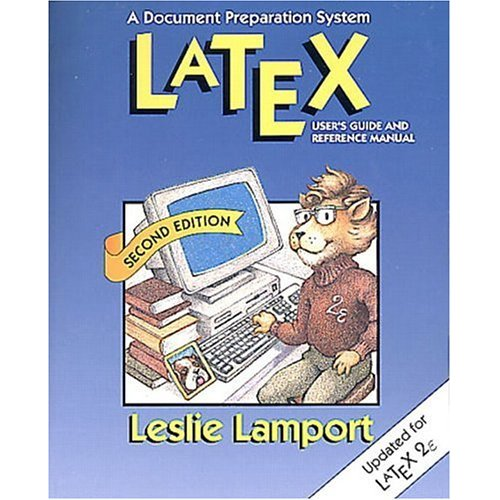
\includegraphics[width=0.3\textwidth]{lamport}
    \caption{The \LaTeX\ ``bible'', 2. edition \label{fig:lamport}}
\end{figure}

There are plenty of good \LaTeX\ editors, and of course, there are many possibilities for the Emacs users\footnote{\url{www.gnu.org/software/emacs}}. Personally, I use {\em texmaker}\footnote{\url{www.xm1math.net/texmaker/}}
for OSX, and 
{\em Kile}\footnote{\url{kile.sourceforge.net}}
for Ubuntu. MS users may try {\em WinEDT}\footnote{\url{www.winedt.com}}. There is also several online options, for instance {\em Overleaf}\footnote{\url{https://www.overleaf.com/}}.

\section{Compilation}

Making documents with \LaTeX\ is basically like writing software. 
This document is produced by compiling a collection of files, all in the same folder.
There is a top level file called 
{\tt main.tex}, which contains commands that decide format, layout etc., or in other words, the {\em style}\footnote{Think of HTML and stylesheets \dots guess where that idea came from \dots}. It also includes the files containing the actual text (in general one file for each chapter).

To compile the document to generate a pdf file, use your terminal/command window (or use the build function in your editor), go to the document folder, and issue this command twice: 

\verb|pdflatex main|

This process produces a  pdf file,
{\tt main.pdf}. When printing this particular document, remember to select the double page option.

However, as you may have experienced when compiling source code, there might be syntax errors, missing files etc. to be fixed. \LaTeX\  is quite verbose when compiling, and does a lot of complaining (warnings), which you most often can ignore. However, it can be a bit tricky to find the source for an error. You sholud typically search backwards from the end of the compilation output. Listing \ref{list:latexerror} is an example from compiling this document, where the error is 
misspelling of the \LaTeX\  macro (should be \verb|\LaTeX|, not \verb|\LateX|). The key error message is \verb|! Undefined control sequence|, followed by a quotation of the line where the error has occurred, along with the line number. The name of current file is found a couple of lines above: \verb|(./how-to.tex|.

\begin{lstlisting}[float=htpb, caption=\LaTeX\ error output,label=list:latexerror]
...

Overfull \hbox (6.0pt too wide) in paragraph at lines 43--44
[][][][][][]

Underfull \hbox (badness 10000) in paragraph at lines 43--44

) (./conclusion.tex [20]
Chapter 7.
[21]) (./main.bbl [22]) [23] [24]
No file main.ind.
(./how-to.tex
Appendix A.
[25]
! Undefined control sequence.
l.48 misspelling of the  \LateX
                         \  macro (should be \verb|\La...

? 
} 
\end{lstlisting} 

\section{Chapters/Sections/Paragraphs}

\LaTeX\  lets you break the document down into chapters, sections, subsections, subsubsections and paragraphs. By default subsubsections and paragraphs are not numbered or included in the table of contents. 

A {\em chapter} may contain plain text, elements like figures and tables, and {\em sections}. 
Plain text is commonly structured by {\em paragraphs}. Paragraphs are separated by one or more {\em empty lines}\footnote{Correspondingly, when there are two or more       consecutive          whitespaces in the text, these will be ignored.}. 
A section may contain {\em subsections}, and the next level is {\em subsubsection}.
Finally we have a special type of {\em paragraph}.

Below follows examples of all these constructs.


\section{Section} 
This is a section. \lipsum[10-12]
\subsection{Sub section} 
This is a sub section. \lipsum[13-14]
\subsubsection{Sub sub section} 
This is a sub sub section. \lipsum[15-16]
\paragraph{Paragraph} 
This is a titled paragraph.
Please note the difference between the standard paragraphs produced by blank lines, and this type, which is the lowest level of elements with titles.

\lipsum[17-18]

\section{Figures, tables, equations, etc.}

Please see the source code ({\tt how-to.tex}) for details on the implementation of these elements.

In general, figures and tables shall be numbered, and have a caption. Numbered figures and tables {\em must} be referenced at least once in the text. Equations and similar elements should also be numbered, but they are not always referred to.

Figures, tables, equations, and similar constructs are so-called {\em floats}. This means that \LaTeX\ will place them in a position that is ``best'', taking many aspects into consideration. The result is that the elements may not be positioned exactly where the author wants (in particular when you have many floats near each other, like in text you are reading now), and this is according to my experience frustrating for the novice user\dots see Section \ref{sec:bestpractise}. Remember to include an empty line in the source prior to the float.

\begin{figure}[!h]
  \begin{center}
    \subfigure[input]{\label{fig:aust}
\includegraphics[width=2.5in]{introaustralia}}
    \subfigure[output]{\label{fig:approx}
\includegraphics[width=2.25in]{australia_approx}}
  \end{center}
  \caption{Input and result from running the Douglas-Peucker line simplification algorithm (from \cite{kjeldsen05cor})}
  \label{fig:dpaustralia}
\end{figure}

Figures are most often produced from files in common graphics formats (like pdf, png, jpg, etc). You can use a single image file, as in Figure \ref{fig:lamport}, or
you can combine several images, see Figure \ref{fig:dpaustralia}, consisting of Figures \ref{fig:aust} and \ref{fig:approx}.

If you want to wrap text around an illustration, the {\tt wrapfig} package can be used, as demonstrated in Figures \ref{fig:wrap-inner} and \ref{fig:wrap-outer}.

\lipsum[92]

\begin{wrapfigure}{i}{0.5\textwidth}
  \centering 
  
\includegraphics[width=0.48\textwidth]{introaustralia}
  \caption{Near inner margin}
  \label{fig:wrap-inner}
\end{wrapfigure}

\lipsum[97]

\begin{wrapfigure}{o}{0.5\textwidth}
  \centering 
  
\includegraphics[width=0.48\textwidth]{introaustralia}
  \caption{Near inner margin}
  \label{fig:wrap-outer}
\end{wrapfigure}

Tables has a relatively steep learning curve.
Still, simple tables, like Table \ref{tab:simple}, are relatively easy to make.
A more complex example is demonstrated in Table \ref{tab:complex}.

\begin{table}[!h]
\centering
\begin{tabular}{c|c|c}
X &  & \\
\hline
& X & \\
\hline
 &  & X \\
\end{tabular}
\caption{Simple table}
\label{tab:simple}
\end{table}

\begin{table}[!h]
\centering
\resizebox{0.6\textwidth}{!}{%
\begin{tabular}{|>{\bfseries}c||p{1.0em}|p{1.0em}|p{1.0em}|p{1.0em} l|}      \hline
\textbf{Combination} &\multicolumn{5}{l|}{\textbf{Included Optional Steps}}\\\cline{2-6}
   & \textbf{1}&\textbf{2}&\textbf{3}&\textbf{4}&\\\hline\hline
 1 & X & & & &    \\\hline
13 &  &  & X & X &\\\hline
14 &  &  &  & X & \\\hline\hline
15 & \multicolumn{4}{l}{Nano Particles Deposited, Not Sintered}&\\\hline
16 & \multicolumn{4}{l}{Only Grinded Wafer 1, No Particles Deposited, Not Sintered}&\\\hline
17 & \multicolumn{4}{l}{Only Grinded Wafer 2, No Particles Deposited, Not Sintered}&\\\hline
\end{tabular}}
\caption{Complex table}
\label{tab:complex}
\end{table}

Within mathematics and natural sciences there is a common belief that \LaTeX\ is unrivaled when it comes to typesetting formulas, equations, and complex specialized notation, as the following examples demonstrate.

You can have inline equations, like this: $ \alpha = \beta \gamma \delta $, or you can typeset them as numbered floats, as in Equation \ref{eq:abc}.
\begin{equation}
  \alpha = \beta \gamma \delta
  \label{eq:abc}
\end{equation}

Equation \ref{eq:mom-inert} is a bit more complicated:

\begin{equation}
  I_{zz} = \int_{-b/2}^{b/2} \int_{-h/2}^{h/2} y^2 dy dx = \frac{b h^3}{12}
  \label{eq:mom-inert}
\end{equation}

There are loads of special characters, like $\approx$, $\pm$,
$\times$, $\div$, $\propto$, $\leq$, $\geq$, $\ll$, $\gg$, $\neq$,
$\nabla$, $\Re$, $\Im$, $\flat$, $\sharp$, $\partial$, $\infty$, and $\heartsuit$.


See the next section for a complete example of a mathematical proof.

\section{Proof of the Area of a Circle Formula}

\newtheorem{prf}{Theorem}

\begin{prf}
The area of circle with radius $r$ is $\pi r^2$.
\end{prf}

\noindent {\bf Proof:} The equation of a circle centered at the
origin is

$$
x^2 + y^2 = r^2,
$$

\noindent where $r$ is the radius.  We  write $y$ in terms of the
variable $x$ and the constant $r$:

$$
\frac{x^2}{r^2} + \frac{y^2}{r^2} = 1
$$
$$
\frac{y}{r} = \sqrt{1-\frac{x^2}{r^2}}
$$
$$
y= r\sqrt {1-\frac{x^2}{r^2}}
$$

By symmetry, the area of a circle centered at the origin is four
times the area of the circle between $(0,0)$ and $(r, 0)$ above the
$x$-axis.  We can integrate to find the area ($A$):

$$
A = 4r\int_0^r \sqrt {1-\frac{x^2}{r^2}}\, dx
$$

To evaluate the antiderivative of $\displaystyle\sqrt
{1-\frac{x^2}{r^2}}$, we make the substitutions:

$$
x = r \sin \theta
$$
$$
\theta = \arcsin \frac{x}{r}
$$
$$
dx = r\cos \theta\, d\theta
$$

Thus, our integral becomes:

$$
A=4r\int_0^r \sqrt {1-\frac{x^2}{r^2}}\, dx = 4r\int_0^{\pi/2}
r\sqrt{1-\sin^2 \theta} \cos \theta\, d\theta
$$

 We can use the trigonometric identity $1 - \sin^2 \theta = \cos^2 \theta$:

$$
A=4r\int_0^{\pi/2} r\sqrt{1-\sin^2 \theta} \cos \theta\, d\theta=
4r^2\int_0^{\pi/2} \cos^2 \theta\, d\theta
$$

We then apply $\cos^2 \theta = \frac{1}{2}(1 + \cos 2\theta)$:

\begin{eqnarray*}
4r^2\int_0^{\pi/2} \cos^2 \theta\, d\theta &=& 4r^2\int_0^{\pi/2}  \frac{1}{2}(1 + \cos 2\theta) \,d\theta\\
& = & {2r^2\theta}\Bigg{|}_0^{\pi/2} + 2r^2\int_0^{\pi/2} \cos 2\theta \,d\theta\\
                                  & = & \pi r^2 + 2r^2(\sin2\theta)\Bigg{|}_0^{\pi/2}\\
                                  & = & \pi r^2
\end{eqnarray*}

Thus, the area of a circle with radius $r$ is $\pi r^2$.\hfill$\blacksquare$

\section{Listings and other {\em environments}}

You can apply specialized layout by using  {\em environments}. Environments are constructed like this:

\begin{lstlisting}[float=htpb]
\begin{some-environment}
The text and other contents goes here
\end{some-environment}
\end{lstlisting}

The most common environments are the following three different list types\footnote{Here we are using compact versions of the standard lists, which tend to produce to much ``air''}. First, the bullet list:

\begin{compactitem}
\item First item
\item Second item
\item Third item
\end{compactitem}
Then, the enumerated list:
\begin{compactenum}
\item First item
\item Second item
\item Third item
\end{compactenum}
And finally the decription list:
\begin{compactdesc}
\item [First item] First description \lipsum[5]
\item [Second item] Second description
\item [Third item] Third description
\end{compactdesc}

Needless to say, as anything else in \LaTeX, these lists can be customized to your liking.

\section{Source code}
\label{sec:sourcecode} 

Large chunks of code should be placed in an appendix, but smaller pieces can be listed in the main part. We here demonstrate two ways of doing this.

In Listing \ref{list:hanoi} we have included code from a separate file.

%\lstinputlisting[caption=Recursive solution of Towers in Hanoi, label=list:hanoi, language=Java,float=htpb]{hanoi.java}
%writelatex.com does not allow to upload *.java files, must use another file extension
\lstinputlisting[caption=Recursive solution of Towers in Hanoi, label=list:hanoi, language=Java,float=htpb]{hanoi.txt}
\index{Recursion|see{Recursion}}
\index{Tower of Hanoi}

In Listing \ref{list:hanoi2} we have copied and pasted from the same file.

\begin{lstlisting}[caption=Core of the recursive solution of Towers in Hanoi,label=list:hanoi2,  language=Java,float=htpb]
// move n smallest discs from one pole to another, using the temp pole
 public static void hanoi(int n, String from, String temp, String to) {
     if (n == 0) return;
     hanoi(n-1, from, to, temp);
     System.out.println(''Move disc '' +n+ '' from '' +from+ '' to '' +to);
     hanoi(n-1, temp, from, to);
}
\end{lstlisting}

\section{Cross-references and bibliography}

As mentioned earlier, all non-text elements should be numbered, and should be referenced to at least once in the text.
This is what is called {\em cross-referencing}, and is easily accomplished.
First we need to attach a label to the element: \verb|\label{type:name}|. Then we use this label in the reference: \verb|\ref{type:name}|. The reference is only a number, so we usually add the element type as a capitalized prefix, for instance like his: \verb|Figure \ref{fig:lamport}}|, which produces: Figure \ref{fig:lamport}.

When you need a reference to an item in your bibliography (books, articles, web sites etc), you need to use one or more ``database'' files, which are plain texts files with bibliography items formatted according to certain rules. These files have the extension {\tt .bib}, and must be included in the main file.
An example of a correctly formatted bibliography item is found in \ref{list:bibtex}.

\begin{lstlisting}[caption=BibTex entry,label=list:bibtex,language=Tex,float=!h]
 @book{perelman97mht,
 author = {Perelman, Leslie and Barrett, Edward},
 title = {{The Mayfield Handbook of Technical and Scientific Writing}},
 year = {1997},
 edition = {1},
 publisher = {McGraw-Hill, Inc.},
 address = {New York, NY, USA},
} 
\end{lstlisting} 

This format is called  {\em bibtex}, and all the academic search engines, including
 {\em Google Scholar}, exports to this format.
When referencing, you use this command: \verb|\cite{perelman97mht}|
and you get: \cite{perelman97mht}. If you want to specify page(s), use \verb|\cite[p. XX]{perelman97mht}|, which results in \cite[p. XX]{perelman97mht}.
 
 To include the references, you run the following sequence:
 
\begin{lstlisting}[float=!ht]
pdflatex main
bibtex main
pdflatex main
\end{lstlisting}

Bibtex generates the final bibliography only from the references in the document (and not from all the items in the {\tt .bib} files).

The different scientific communities have their own guidelines for how to format the entries in the bibliography, and how to format the references in the document.
You decide which style to use with the command \verb|\bibliographystyle{somestyle}| in the main file.

There are several tools for creating and maintaining bibliography databases that export bibtex files, both standalone programs, plugins to editors and browsers, and cloud based services\footnote{For instance, check out \url{zotero.org}}.

\section{Glossary}

You may also make a glossary page, where the terms have descriptions and lists of pages they occur on. You need to provide the terms and their descriptions in the preamble, for instance in a separate file, see \verb|glossary.tex|. An entry looks like this:

\begin{lstlisting}[float,float=!h]
\newglossaryentry{maths}
{
    name=mathematics,
    description={Mathematics is what mathematicians do}
}
\end{lstlisting}

The terms are marked in the text like this:  
\gls{maths}. The glossary is produced by including \verb|\\printglossaries| in the main file, and run \verb|makeglossaries| when compiling. The index page is produced by including \verb|\printindex| in the main file, and running the following sequence:

\begin{lstlisting}[float,float=!h]
pdflatex main
makeglossary main
pdflatex main
\end{lstlisting}

The result in the glossary will be something like this:  ``mathematics Mathematics is what mathematicians do. 1, 29''.

\section{Fonts}

Fore every  \LaTeX\ distribution, there is a default set of fonts.
It is possible to customize this  setup.
Don't\footnote{It's by all means possible, but if you get this urge, you most likely suffer from a stroke of extreme procrastination \dots ah \dots well, then, check out the very last part of the preamble (that is everything before {\tt begin{document}} in the main file).}.

You can do it locally like this (but use it with extreme care):

{\fontfamily{pzc}\selectfont \lipsum[21]}

However, size, weight, style and font family may be manipulated using the following standard commands.

\paragraph{Font size}

First of all, you decide in the preamble the default font size for your document. The {\tt documentclass} takes the parameters {\tt 10pt},  {\tt 11pt},  or {\tt 12pt}. Locally, you can change the style by the following commands, that resizes the font {\em relatively} to the default size:

    \tiny tiny
    
    \scriptsize scriptsize
    
    \footnotesize footnotesize
    
    \small small
    
    \normalsize Default: normalsize
    
    \large  large
    
    \Large Large
    
    \LARGE LARGE
    
    \huge huge
    
    \Huge  Huge
    
    \normalsize 
    
\paragraph{Font weight (Font series)}
You can locally change the font weight:
    
    \textmd{Default: Medium}
    
    \textbf{Bold}
    
    
\paragraph{Font style (Font shape)}
You can locally change the font style:
    
    \textup{Default: Normal (Upright/Roman)}
    
    \textit{Italic}
    
    \textsl{Slanted}
    
    \textsc{Small caps}
    
\paragraph{Font family}
You can locally change the font family:
    
    \textrm{Default: Roman (serif)}
    
    \textsf{Sans serif}
    
    \texttt{Typewriter (monospace)}


\section{Best practice}
\label{sec:bestpractise}

\begin{compactitem}
\item First: Focus on {\em content} and {\em structure} 
\item Later: Decide on layout and style
\item Use mostly the default settings
\item If you need special functionality, look for packages covering your needs
\item If you do not find suitable packages, make your own macros
\item Learn by 1) asking fellow students, 2) google and cut'n paste, and 3) by sending me an email or come to my office
\item Compile frequently
\item Commit frequently to your versioning system\footnote{SVN is a good choice, or use any of the many free online services.}
\item Run spell checks when things start to get complete\footnote{Most editors provide built-in spell check functionality (which ignores the markup commands).  On Linux platforms you have the ispell and aspell command line tools which can be configured for \LaTeX. There are also stand-alone tools around.}
\item When the document absolutely complete: perform minor fine-tuning (typically to sort out bad placements of floats). Remember that every fix you apply may affect the subsequent layout.
\end{compactitem}



              % READ THIS CHAPTER: Sample code of everything you need and more :-)

\end{document}
